\section{Package dto}
Per la composizione delle richieste che il client invia o delle risposte che il server manda, sono state create vari tipi di requests e responses.\\
Ogni oggetto di risposta è composto da un oggetto data e un oggetto metadata, mentre gli oggetti di richiesta possono variare. Se la richiesta è fatta per un endpoint che restituisce una lista di risultati, possiamo avere tre casistiche:
\begin{itemize}
\item body\textsubscript{g} formato da un oggetto data, contenente informazioni utili alla risposta, e metadata che contiene i dati di paginazione\textsubscript{g};
\item nessun body, ma soltanto i dati di paginazione passati come parametri di query\textsubscript{g};
\item path variable\textsubscript{g} che solitamente fa riferimento ad un ID, nei parametri di query e dati di paginazione.
\end{itemize}
Se invece la richiesta è costruita per un endpoint che restituisce un singolo oggetto nell'oggetto data, non viene utilizzato alcun body o parametri di query, ma solo una path variable.\\
Questa suddivisione data e metadata è un modello comune nella progettazione API per separare i dati effettivi o dati che forniscono informazioni per ottenere un tipo di risposta, dalle informazioni aggiuntive che descrivono il risultato o aggiungono caratteristiche alla richiesta.\\
Questo package è formato da vari subpackage\textsubscript{g}.
\subsection{Common}
\begin{figure}[H] 
    \centering 
    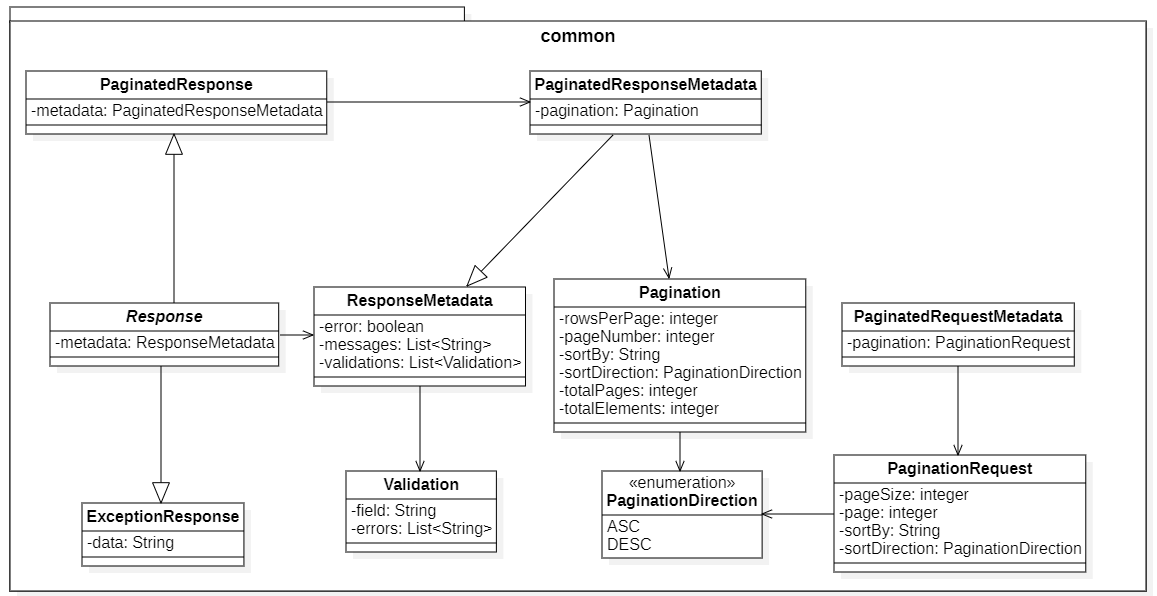
\includegraphics[width=1.0\columnwidth]{dto-sub-common} 
    \caption{Subpackage common}
\end{figure}
Questo subpackage contiene la response di base, response paginata, la response utilizzata nell'eccezione personalizzata, una request per la paginazione e i vari metadata utilizzati nelle responses. Ogni metadata contiene un boolean che indica se si è andati in errore (true) o meno (false), il messaggio di errore e una lista di \texttt{validation}, contenente informazioni di validazione dei dati.\\
È stata creata una classe \texttt{Pagination} per avere un controllo personalizzato sulla Paginazione.
\subsection{Requests e Body}
\begin{figure}[H] 
    \centering 
    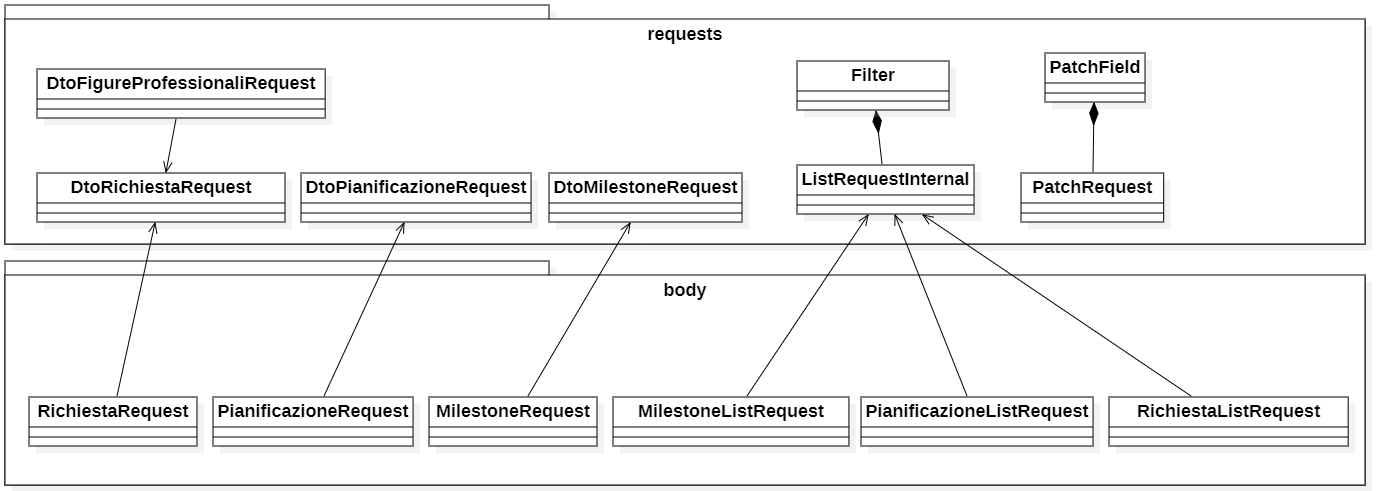
\includegraphics[width=1.0\columnwidth]{dto-sub-requests-body-2} 
    \caption{Subpackage requests e body}
\end{figure}
Questi due subpackages sono correlati tra di loro dato che ogni body ha come attributo una request presa dal subpackage requests.
Esistono due tipi di body:
\begin{itemize}
\item ogni \texttt{Request} singola contiene una request DTO formata dai campi utili che l'utente deve inserire per eseguire un determinato endpoint;
\item ogni \texttt{ListRequest} è formata da un oggetto data di tipo \texttt{ListRequestInternal}, che contiene tre parametri: filters, lista di oggetti Filter formati da campo-valore, una stringa q (quicksearch) utile nella query personalizzata per cercare in determinati campi quello che l'utente inserisce e infine andOperator per impostare i filtri in And o in Or nella query. 
\end{itemize}
All'interno del subpackage requests troviamo anche \texttt{PatchRequest}, contenente un unico campo corrispondente ad una lista di \texttt{PatchField}. Questa richiesta viene utilizzata nella richieste PATCH, in cui è possibile inserire uno o più valori in base a cosa si va a modificare.

\subsection{Responses}
\begin{figure}[H] 
    \centering 
    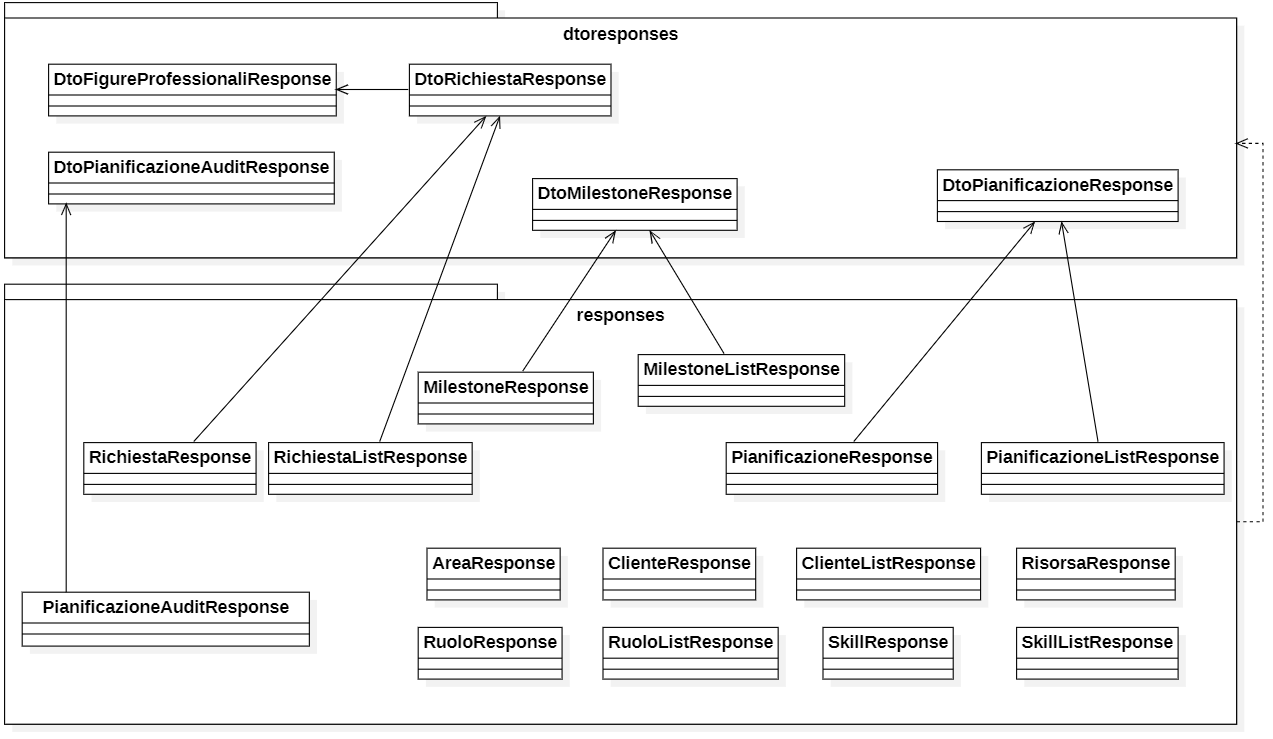
\includegraphics[width=0.9\columnwidth]{dto-sub-responses} 
    \caption{Subpackage responses e dtoresponses}
\end{figure}
Il package responses contiene tutte le response per entità. Ogni response eredita la classe astratta \texttt{response} se è una risposta singola, altrimenti eredita la classe \texttt{PaginatedResponse} se è una lista di risposte. Questo permette all'utente di visualizzare la risposta dopo aver interagito con un'endpoint, formata da data e metadata.\\
Ogni response contiene un solo attributo che corrisponde all'oggetto data e può essere una responses DTO del subpackage dtoresponses o un'entità DTO del subpackage delle entità. Se si è di fronte ad una \texttt{ListResponse} l'attributo sarà una lista, altrimenti un oggetto singolo.